\section{Arbeid}

\subsection{Wat is arbeid?}
Arbeid is een vorm van energieoverdracht die plaatsvindt wanneer een kracht wordt uitgeoefend op een object en het object zich verplaatst in de richting van die kracht.
In de context van thermische fysica, wordt arbeid vaak geassocieerd met processen waarbij een systeem energie verliest of wint door middel van mechanische interacties.

\begin{definition}
    \textbf{Uitwendige Arbeid}: Arbeid die wordt verricht door een systeem op zijn omgeving, of door de omgeving op het systeem, als gevolg van mechanische interacties.
\end{definition}
\medskip
\begin{definition}
    \textbf{Inwendige Arbeid}: Arbeid die wordt verricht binnen een systeem, als gevolg van interne krachten en processen. \footnote{Een warme bal maakt nog steeds dezelfde beweging als een koude bal, maar er is wel een verschil in de interne energie, dus een verschil in inwendige arbeid.}
\end{definition}
\medskip
\begin{definition}
    \textbf{Positieve Arbeid}: Arbeid verricht op een systeem door zijn omgeving. \(\vec{e}_r = \vec{e}_F\)
\end{definition}
\medskip
\begin{definition}
    \textbf{Negatieve Arbeid}: Arbeid verricht door een systeem op zijn omgeving. \(\vec{e}_r = -\vec{e}_F\)
\end{definition}

\subsection{Arbeid bij volumeverandering}

\begin{figure}[ht]
    \centering
    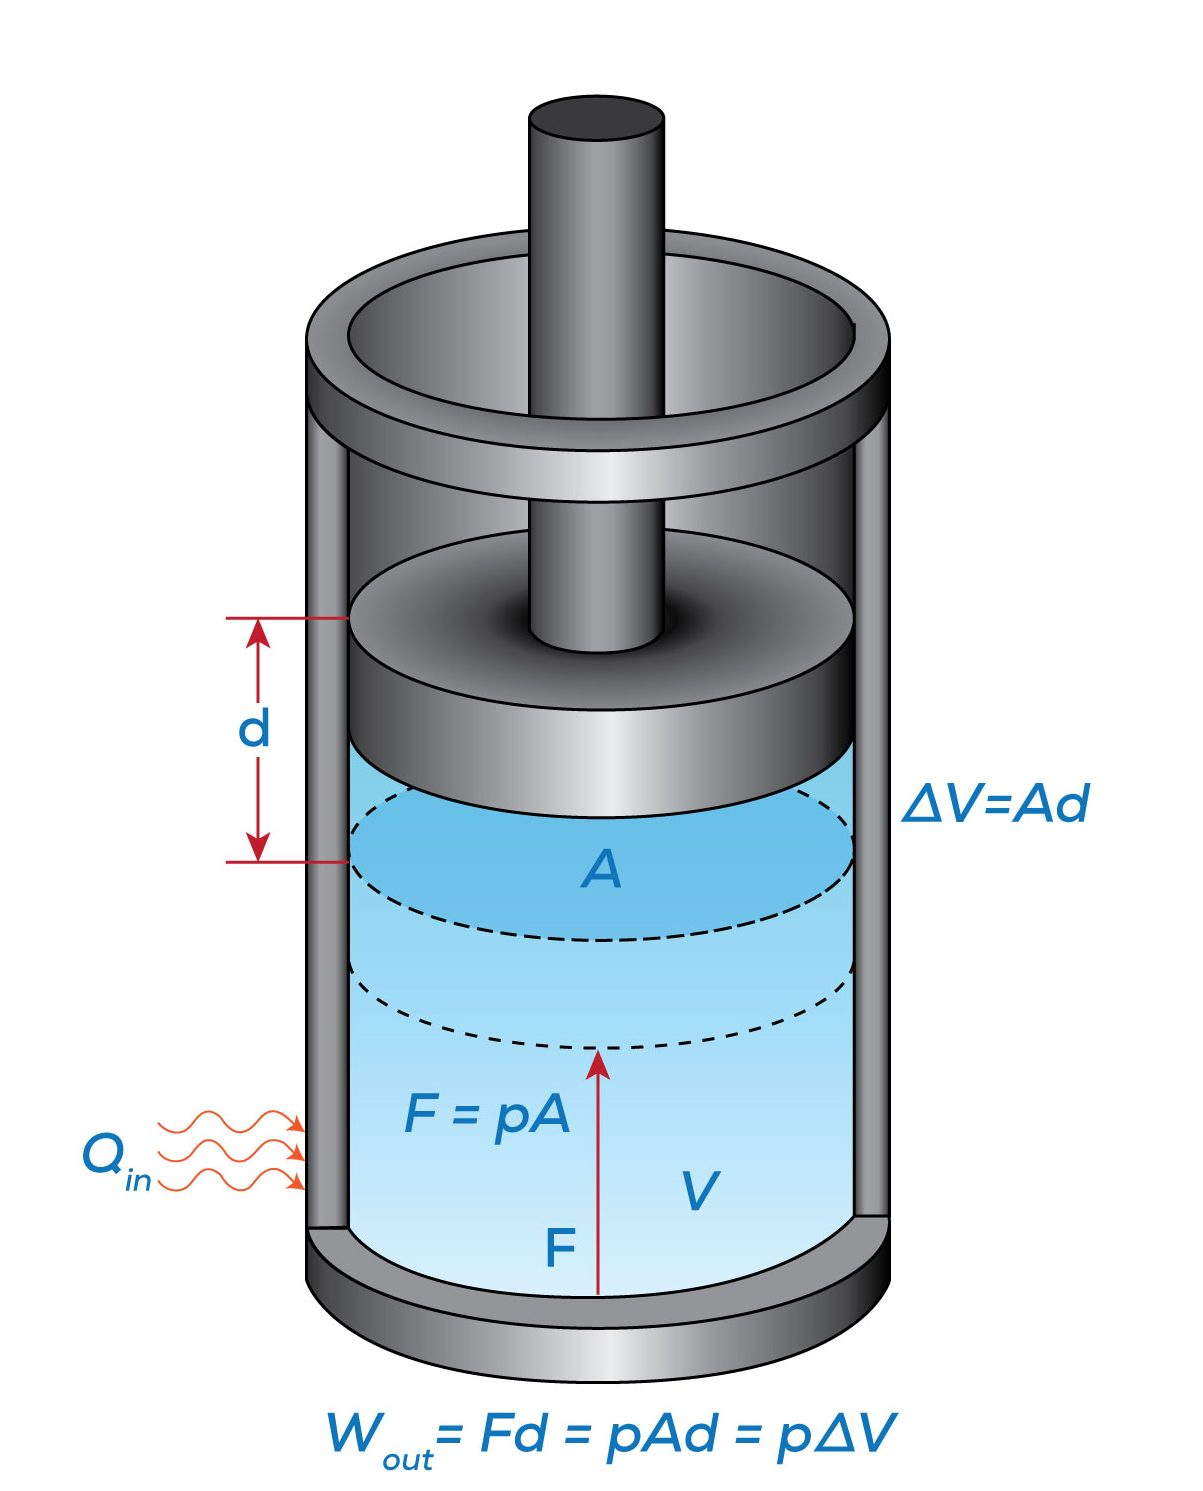
\includegraphics[width=0.3\textwidth]{Foto's-Figuren/Fig.-4-4_boundary-work1-e1626459353689.jpg}
    \caption{Arbeid verricht door een gas tijdens compressie. De kracht \(F\) werkt op de zuiger, waardoor deze zich verplaatst met een afstand \(dx\). De arbeid \(dW\) wordt gegeven door \(dW = F \cdot dx\). \footnotesize \copyright{Kh1604 is licensed under a CC BY-SA (Attribution ShareAlike) license}}
    \label{fig:work-gas-compression}
\end{figure}

\[
dW = F \cdot dx = -PAdx = -PdV
\]

Een negatief teken betekent dat een volumevergroting gepaard gaat met een negatieve arbeid, terwijl een volumeverkleining gepaard gaat met een positieve arbeid. 

Voor een quasistatisch proces geldt:
\begin{equation}
    \label{eq:hydrostatische-arbeid-algemeen}
    W = - \int_{V_i}^{V_f} PdV
\end{equation}

\begin{figure}[ht]
    \centering
    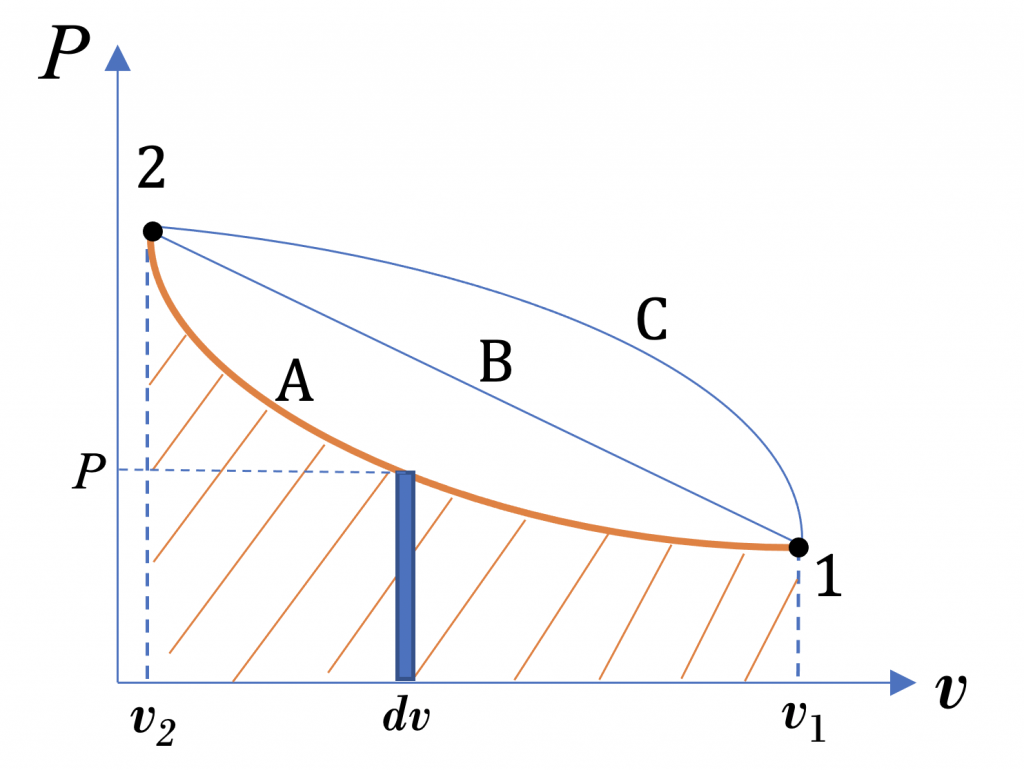
\includegraphics[width=0.3\textwidth]{Foto's-Figuren/P-v-for-boundary-work-1024x770.png}
    \caption{PV-diagram van een gas. De arbeid verricht door het gas tijdens een proces wordt gegeven door de oppervlakte onder de curve in het PV-diagram. \footnotesize \copyright{ Kh1604 is licensed under a CC BY-SA (Attribution ShareAlike) license}}
    \label{fig:work-gas-pv}
\end{figure}

Voor een quasistatisch proces is de arbeid gelijk aan de oppervlakte onder de curve in het PV-diagram. Stel we gaan van punt i naar punt f met een volume compressie:
\[
W_{if} = - \int_{V_i}^{V_f} PdV
\]
Als we van dat punt terug gaan van punt f naar punt i (en dus eeen volume expansie hebben), dan is de arbeid:
\[
W_{fi} = - \int_{V_f}^{V_i} PdV
\]
Dit betekend dat we een cyclus kunnen maken waarbij geldt \(W_{if} = -W_{fi}\). Dit is voor een quasistatisch proces langs heetzelfde pad!

Onze conventie voor cyclussen is als volgt: wijzerzin betekend dat er negatieve arbeid wordt verricht, terwijl tegenwijzerzin betekend dat er positieve arbeid wordt verricht op het systeem. Typisch zijn koelmachines tegenwijzerzin, terwijl warmtemachines wijzerzin zijn.

\subsection{Padafhankelijke Arbeid}

\begin{derivation}
    \textbf{Arbeid is padafhankelijk}: Stel we kunnen van punt 1 naar punt 2 gaan via twee verschillende paden, namelijk pad A en pad C. (Zie figuur \ref{fig:work-gas-pv}.)
    We kunnen ook een cyclus maken door van punt 1 naar punt 2 te gaan via pad C, en vervolgens terug te gaan van punt 2 naar punt 1 via pad A. De netto arbeid verricht tijdens deze cyclus is:
    \begin{align*}
        W_{cyclus} &= W_{21}(C) + W_{12}(A) 
        = -|W_{21}(C)| + |W_{12}(A)| < 0 
        \implies |W_{21}(C)| > |W_{12}(A)| \\
    \end{align*}
    Als we nu proces A van 2 naar 1 laten verlopen, dan is de netto arbeid:
    \begin{align*}
        W_{21}(A) &= -W_{12}(A) <0 \implies |W_{21}(A)| = |W_{12}(A)| \\ 
    \end{align*}
    Uit \(|W_{21}(C)| > |W_{12}(A)|\) en \(|W_{21}(A)| = |W_{12}(A)|\) volgt dat \(|W_{21}(C)| > |W_{21}(A)|\). (Of stel dat beide negatief zijn, dan is \(W_{21}(C) < W_{21}(A)\).)
    Dit betekent dat de arbeid die wordt verricht tijdens het proces van 2 naar 1 via pad C groter is dan de arbeid die wordt verricht tijdens het proces van 2 naar 1 via pad A.
    \qed
\end{derivation}
\medskip
\begin{postulate}
    \textbf{Arbeid is padafhankelijk!}
\end{postulate}

Stel we hebben een  \textbf{isobaar} proces, dan wordt de arbeid:
\begin{equation}
\label{eq: isobare-arbeid}
W = -P \int_{V_i}^{V_f} dV = -P(V_f - V_i) \qquad (P = cst)
\end{equation}
Voor een  \textbf{isochoor} proces is de arbeid triviaal 0.

\textbf{Isotherme arbeid} is dan weer een ander verhaal:
\[
W = - \int_{V_i}^{V_f} P(V)dV
\]
Waarbij de toestandsfunctie \(P(V, T)\) nu enkel van het volume afhangt \(P(V)\). 
Voor een ideaal gas is \(P = \frac{nRT}{V}\), dus de arbeid wordt:
\begin{equation}
\label{eq: isotherme-arbeid-ideaal-gas}
W = - \int_{V_i}^{V_f} \frac{nRT}{V}dV = -nRT \ln\left( \frac{V_f}{V_i} \right) \qquad (T = cst)
\end{equation} 

\textbf{Isotherme toename van druk op een vaste stof}
\[
dV = \left( \frac{\partial V}{\partial P} \right)_T dP = - \kappa V dP \qquad (T = cst)
\]
Waaruit volgt dat de arbeid:
\begin{equation}
\label{eq: isotherme-arbeid-vast-stof}
W = - \int_{P_i}^{P_f} \kappa VP  dP \qquad (T = cst)
\end{equation} 
